\documentclass[1p]{elsarticle_modified}
%\bibliographystyle{elsarticle-num}

%\usepackage[colorlinks]{hyperref}
%\usepackage{abbrmath_seonhwa} %\Abb, \Ascr, \Acal ,\Abf, \Afrak
\usepackage{amsfonts}
\usepackage{amssymb}
\usepackage{amsmath}
\usepackage{amsthm}
\usepackage{scalefnt}
\usepackage{amsbsy}
\usepackage{kotex}
\usepackage{caption}
\usepackage{subfig}
\usepackage{color}
\usepackage{graphicx}
\usepackage{xcolor} %% white, black, red, green, blue, cyan, magenta, yellow
\usepackage{float}
\usepackage{setspace}
\usepackage{hyperref}

\usepackage{tikz}
\usetikzlibrary{arrows}

\usepackage{multirow}
\usepackage{array} % fixed length table
\usepackage{hhline}

%%%%%%%%%%%%%%%%%%%%%
\makeatletter
\renewcommand*\env@matrix[1][\arraystretch]{%
	\edef\arraystretch{#1}%
	\hskip -\arraycolsep
	\let\@ifnextchar\new@ifnextchar
	\array{*\c@MaxMatrixCols c}}
\makeatother %https://tex.stackexchange.com/questions/14071/how-can-i-increase-the-line-spacing-in-a-matrix
%%%%%%%%%%%%%%%

\usepackage[normalem]{ulem}

\newcommand{\msout}[1]{\ifmmode\text{\sout{\ensuremath{#1}}}\else\sout{#1}\fi}
%SOURCE: \msout is \stkout macro in https://tex.stackexchange.com/questions/20609/strikeout-in-math-mode

\newcommand{\cancel}[1]{
	\ifmmode
	{\color{red}\msout{#1}}
	\else
	{\color{red}\sout{#1}}
	\fi
}

\newcommand{\add}[1]{
	{\color{blue}\uwave{#1}}
}

\newcommand{\replace}[2]{
	\ifmmode
	{\color{red}\msout{#1}}{\color{blue}\uwave{#2}}
	\else
	{\color{red}\sout{#1}}{\color{blue}\uwave{#2}}
	\fi
}

\newcommand{\Sol}{\mathcal{S}} %segment
\newcommand{\D}{D} %diagram
\newcommand{\A}{\mathcal{A}} %arc


%%%%%%%%%%%%%%%%%%%%%%%%%%%%%5 test

\def\sl{\operatorname{\textup{SL}}(2,\Cbb)}
\def\psl{\operatorname{\textup{PSL}}(2,\Cbb)}
\def\quan{\mkern 1mu \triangleright \mkern 1mu}

\theoremstyle{definition}
\newtheorem{thm}{Theorem}[section]
\newtheorem{prop}[thm]{Proposition}
\newtheorem{lem}[thm]{Lemma}
\newtheorem{ques}[thm]{Question}
\newtheorem{cor}[thm]{Corollary}
\newtheorem{defn}[thm]{Definition}
\newtheorem{exam}[thm]{Example}
\newtheorem{rmk}[thm]{Remark}
\newtheorem{alg}[thm]{Algorithm}

\newcommand{\I}{\sqrt{-1}}
\begin{document}

%\begin{frontmatter}
%
%\title{Boundary parabolic representations of knots up to 8 crossings}
%
%%% Group authors per affiliation:
%\author{Yunhi Cho} 
%\address{Department of Mathematics, University of Seoul, Seoul, Korea}
%\ead{yhcho@uos.ac.kr}
%
%
%\author{Seonhwa Kim} %\fnref{s_kim}}
%\address{Center for Geometry and Physics, Institute for Basic Science, Pohang, 37673, Korea}
%\ead{ryeona17@ibs.re.kr}
%
%\author{Hyuk Kim}
%\address{Department of Mathematical Sciences, Seoul National University, Seoul 08826, Korea}
%\ead{hyukkim@snu.ac.kr}
%
%\author{Seokbeom Yoon}
%\address{Department of Mathematical Sciences, Seoul National University, Seoul, 08826,  Korea}
%\ead{sbyoon15@snu.ac.kr}
%
%\begin{abstract}
%We find all boundary parabolic representation of knots up to 8 crossings.
%
%\end{abstract}
%\begin{keyword}
%    \MSC[2010] 57M25 
%\end{keyword}
%
%\end{frontmatter}

%\linenumbers
%\tableofcontents
%
\newcommand\colored[1]{\textcolor{white}{\rule[-0.35ex]{0.8em}{1.4ex}}\kern-0.8em\color{red} #1}%
%\newcommand\colored[1]{\textcolor{white}{ #1}\kern-2.17ex	\textcolor{white}{ #1}\kern-1.81ex	\textcolor{white}{ #1}\kern-2.15ex\color{red}#1	}

{\Large $\underline{12a_{0259}~(K12a_{0259})}$}

\setlength{\tabcolsep}{10pt}
\renewcommand{\arraystretch}{1.6}
\vspace{1cm}\begin{tabular}{m{100pt}>{\centering\arraybackslash}m{274pt}}
\multirow{5}{120pt}{
	\centering
	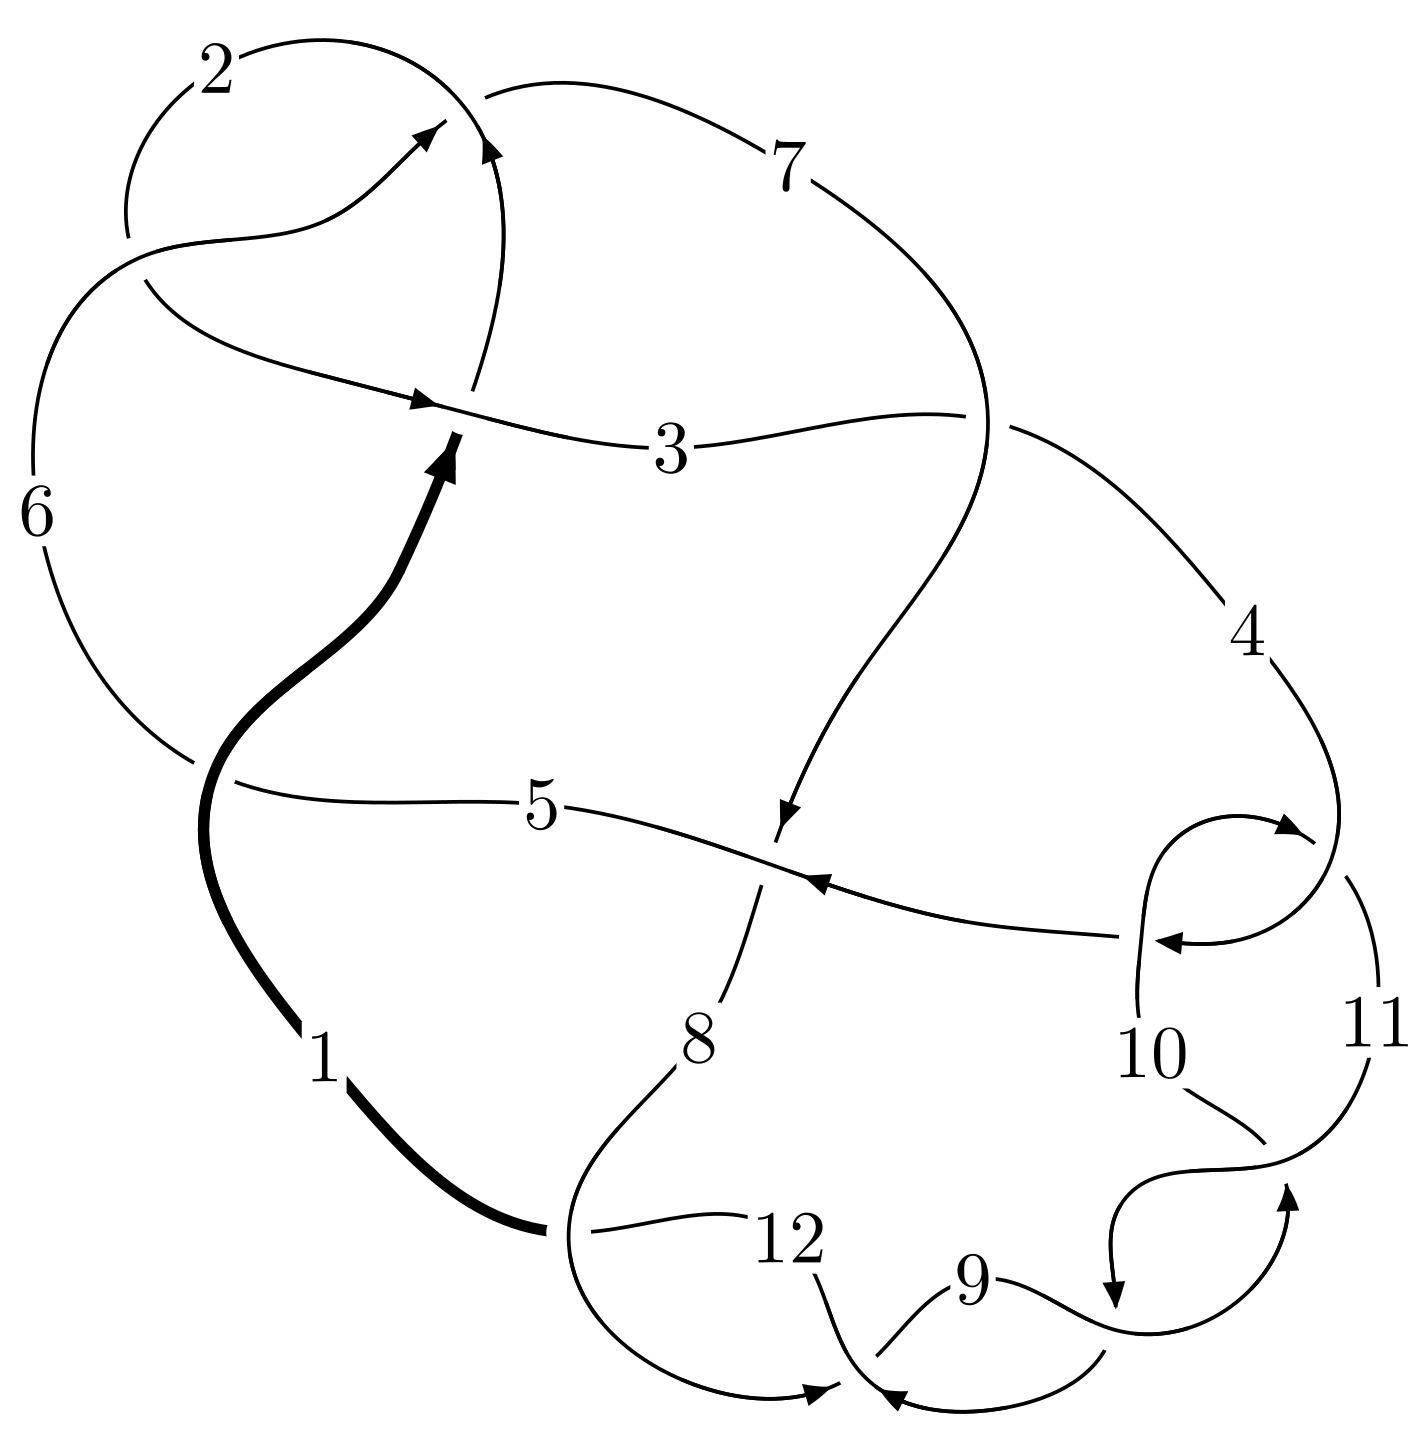
\includegraphics[width=112pt]{../../../GIT/diagram.site/Diagrams/png/1060_12a_0259.png}\\
\ \ \ A knot diagram\footnotemark}&
\allowdisplaybreaks
\textbf{Linearized knot diagam} \\
\cline{2-2}
 &
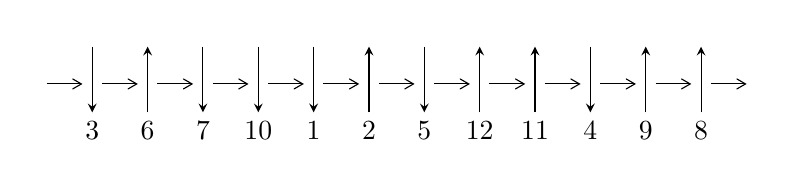
\begin{tikzpicture}[x=20pt, y=17pt]
	% nodes
	\node (C0) at (0, 0) {};
	\node (C1) at (1, 0) {};
	\node (C1U) at (1, +1) {};
	\node (C1D) at (1, -1) {3};

	\node (C2) at (2, 0) {};
	\node (C2U) at (2, +1) {};
	\node (C2D) at (2, -1) {6};

	\node (C3) at (3, 0) {};
	\node (C3U) at (3, +1) {};
	\node (C3D) at (3, -1) {7};

	\node (C4) at (4, 0) {};
	\node (C4U) at (4, +1) {};
	\node (C4D) at (4, -1) {10};

	\node (C5) at (5, 0) {};
	\node (C5U) at (5, +1) {};
	\node (C5D) at (5, -1) {1};

	\node (C6) at (6, 0) {};
	\node (C6U) at (6, +1) {};
	\node (C6D) at (6, -1) {2};

	\node (C7) at (7, 0) {};
	\node (C7U) at (7, +1) {};
	\node (C7D) at (7, -1) {5};

	\node (C8) at (8, 0) {};
	\node (C8U) at (8, +1) {};
	\node (C8D) at (8, -1) {12};

	\node (C9) at (9, 0) {};
	\node (C9U) at (9, +1) {};
	\node (C9D) at (9, -1) {11};

	\node (C10) at (10, 0) {};
	\node (C10U) at (10, +1) {};
	\node (C10D) at (10, -1) {4};

	\node (C11) at (11, 0) {};
	\node (C11U) at (11, +1) {};
	\node (C11D) at (11, -1) {9};

	\node (C12) at (12, 0) {};
	\node (C12U) at (12, +1) {};
	\node (C12D) at (12, -1) {8};
	\node (C13) at (13, 0) {};

	% arrows
	\draw[->,>={angle 60}]
	(C0) edge (C1) (C1) edge (C2) (C2) edge (C3) (C3) edge (C4) (C4) edge (C5) (C5) edge (C6) (C6) edge (C7) (C7) edge (C8) (C8) edge (C9) (C9) edge (C10) (C10) edge (C11) (C11) edge (C12) (C12) edge (C13) ;	\draw[->,>=stealth]
	(C1U) edge (C1D) (C2D) edge (C2U) (C3U) edge (C3D) (C4U) edge (C4D) (C5U) edge (C5D) (C6D) edge (C6U) (C7U) edge (C7D) (C8D) edge (C8U) (C9D) edge (C9U) (C10U) edge (C10D) (C11D) edge (C11U) (C12D) edge (C12U) ;
	\end{tikzpicture} \\
\hhline{~~} \\& 
\textbf{Solving Sequence} \\ \cline{2-2} 
 &
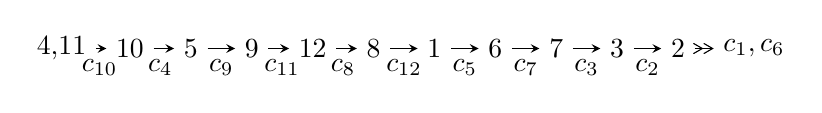
\begin{tikzpicture}[x=22pt, y=7pt]
	% node
	\node (A0) at (-1/8, 0) {4,11};
	\node (A1) at (1, 0) {10};
	\node (A2) at (2, 0) {5};
	\node (A3) at (3, 0) {9};
	\node (A4) at (4, 0) {12};
	\node (A5) at (5, 0) {8};
	\node (A6) at (6, 0) {1};
	\node (A7) at (7, 0) {6};
	\node (A8) at (8, 0) {7};
	\node (A9) at (9, 0) {3};
	\node (A10) at (10, 0) {2};
	\node (C1) at (1/2, -1) {$c_{10}$};
	\node (C2) at (3/2, -1) {$c_{4}$};
	\node (C3) at (5/2, -1) {$c_{9}$};
	\node (C4) at (7/2, -1) {$c_{11}$};
	\node (C5) at (9/2, -1) {$c_{8}$};
	\node (C6) at (11/2, -1) {$c_{12}$};
	\node (C7) at (13/2, -1) {$c_{5}$};
	\node (C8) at (15/2, -1) {$c_{7}$};
	\node (C9) at (17/2, -1) {$c_{3}$};
	\node (C10) at (19/2, -1) {$c_{2}$};
	\node (A11) at (45/4, 0) {$c_{1},c_{6}$};

	% edge
	\draw[->,>=stealth]	
	(A0) edge (A1) (A1) edge (A2) (A2) edge (A3) (A3) edge (A4) (A4) edge (A5) (A5) edge (A6) (A6) edge (A7) (A7) edge (A8) (A8) edge (A9) (A9) edge (A10) ;
	\draw[->>,>={angle 60}]	
	(A10) edge (A11);
\end{tikzpicture} \\ 

\end{tabular} \\

\footnotetext{
The image of knot diagram is generated by the software ``\textbf{Draw programme}" developed by Andrew Bartholomew(\url{http://www.layer8.co.uk/maths/draw/index.htm\#Running-draw}), where we modified some parts for our purpose(\url{https://github.com/CATsTAILs/LinksPainter}).
}\phantom \\ \newline 
\centering \textbf{Ideals for irreducible components\footnotemark of $X_{\text{par}}$} 
 
\begin{align*}
I^u_{1}&=\langle 
u^{55}+5 u^{53}+\cdots+2 u-1\rangle \\
I^u_{2}&=\langle 
u^2+u+1\rangle \\
\\
\end{align*}
\raggedright * 2 irreducible components of $\dim_{\mathbb{C}}=0$, with total 57 representations.\\
\footnotetext{All coefficients of polynomials are rational numbers. But the coefficients are sometimes approximated in decimal forms when there is not enough margin.}
\newpage
\renewcommand{\arraystretch}{1}
\centering \section*{I. $I^u_{1}= \langle u^{55}+5 u^{53}+\cdots+2 u-1 \rangle$}
\flushleft \textbf{(i) Arc colorings}\\
\begin{tabular}{m{7pt} m{180pt} m{7pt} m{180pt} }
\flushright $a_{4}=$&$\begin{pmatrix}0\\u\end{pmatrix}$ \\
\flushright $a_{11}=$&$\begin{pmatrix}1\\0\end{pmatrix}$ \\
\flushright $a_{10}=$&$\begin{pmatrix}1\\- u^2\end{pmatrix}$ \\
\flushright $a_{5}=$&$\begin{pmatrix}- u\\u^3+u\end{pmatrix}$ \\
\flushright $a_{9}=$&$\begin{pmatrix}u^2+1\\- u^2\end{pmatrix}$ \\
\flushright $a_{12}=$&$\begin{pmatrix}u^4+u^2+1\\- u^4\end{pmatrix}$ \\
\flushright $a_{8}=$&$\begin{pmatrix}u^6+u^4+2 u^2+1\\- u^6- u^2\end{pmatrix}$ \\
\flushright $a_{1}=$&$\begin{pmatrix}u^8+u^6+3 u^4+2 u^2+1\\- u^8-2 u^4\end{pmatrix}$ \\
\flushright $a_{6}=$&$\begin{pmatrix}- u^{19}-2 u^{17}-8 u^{15}-12 u^{13}-21 u^{11}-22 u^9-20 u^7-12 u^5-5 u^3-2 u\\u^{19}+u^{17}+6 u^{15}+5 u^{13}+11 u^{11}+7 u^9+6 u^7+2 u^5+u^3+u\end{pmatrix}$ \\
\flushright $a_{7}=$&$\begin{pmatrix}u^{10}+u^8+4 u^6+3 u^4+3 u^2+1\\- u^{12}-2 u^{10}-4 u^8-6 u^6-3 u^4-2 u^2\end{pmatrix}$ \\
\flushright $a_{3}=$&$\begin{pmatrix}u^{21}+2 u^{19}+\cdots+6 u^3+u\\- u^{23}-3 u^{21}+\cdots-2 u^3+u\end{pmatrix}$ \\
\flushright $a_{2}=$&$\begin{pmatrix}- u^{52}-5 u^{50}+\cdots+3 u^2+1\\u^{54}+6 u^{52}+\cdots-4 u^4+u^2\end{pmatrix}$\\&\end{tabular}
\flushleft \textbf{(ii) Obstruction class $= -1$}\\~\\
\flushleft \textbf{(iii) Cusp Shapes $= -4 u^{54}-4 u^{53}+\cdots+16 u-6$}\\~\\
\newpage\renewcommand{\arraystretch}{1}
\flushleft \textbf{(iv) u-Polynomials at the component}\newline \\
\begin{tabular}{m{50pt}|m{274pt}}
Crossings & \hspace{64pt}u-Polynomials at each crossing \\
\hline $$\begin{aligned}c_{1}\end{aligned}$$&$\begin{aligned}
&u^{55}+30 u^{54}+\cdots-2 u-1
\end{aligned}$\\
\hline $$\begin{aligned}c_{2},c_{6}\end{aligned}$$&$\begin{aligned}
&u^{55}-2 u^{54}+\cdots-4 u+1
\end{aligned}$\\
\hline $$\begin{aligned}c_{3},c_{5}\end{aligned}$$&$\begin{aligned}
&u^{55}+2 u^{54}+\cdots+20 u+1
\end{aligned}$\\
\hline $$\begin{aligned}c_{4},c_{10}\end{aligned}$$&$\begin{aligned}
&u^{55}+5 u^{53}+\cdots+2 u+1
\end{aligned}$\\
\hline $$\begin{aligned}c_{7}\end{aligned}$$&$\begin{aligned}
&u^{55}-10 u^{54}+\cdots-10716 u+797
\end{aligned}$\\
\hline $$\begin{aligned}c_{8},c_{9},c_{11}\\c_{12}\end{aligned}$$&$\begin{aligned}
&u^{55}-10 u^{54}+\cdots-2 u+1
\end{aligned}$\\
\hline
\end{tabular}\\~\\
\newpage\renewcommand{\arraystretch}{1}
\flushleft \textbf{(v) Riley Polynomials at the component}\newline \\
\begin{tabular}{m{50pt}|m{274pt}}
Crossings & \hspace{64pt}Riley Polynomials at each crossing \\
\hline $$\begin{aligned}c_{1}\end{aligned}$$&$\begin{aligned}
&y^{55}-10 y^{54}+\cdots-10 y-1
\end{aligned}$\\
\hline $$\begin{aligned}c_{2},c_{6}\end{aligned}$$&$\begin{aligned}
&y^{55}+30 y^{54}+\cdots-2 y-1
\end{aligned}$\\
\hline $$\begin{aligned}c_{3},c_{5}\end{aligned}$$&$\begin{aligned}
&y^{55}-50 y^{54}+\cdots+94 y-1
\end{aligned}$\\
\hline $$\begin{aligned}c_{4},c_{10}\end{aligned}$$&$\begin{aligned}
&y^{55}+10 y^{54}+\cdots-2 y-1
\end{aligned}$\\
\hline $$\begin{aligned}c_{7}\end{aligned}$$&$\begin{aligned}
&y^{55}-30 y^{54}+\cdots+41338098 y-635209
\end{aligned}$\\
\hline $$\begin{aligned}c_{8},c_{9},c_{11}\\c_{12}\end{aligned}$$&$\begin{aligned}
&y^{55}+70 y^{54}+\cdots-26 y-1
\end{aligned}$\\
\hline
\end{tabular}\\~\\
\newpage\flushleft \textbf{(vi) Complex Volumes and Cusp Shapes}
$$\begin{array}{c|c|c}  
\text{Solutions to }I^u_{1}& \I (\text{vol} + \sqrt{-1}CS) & \text{Cusp shape}\\
 \hline 
\begin{aligned}
u &= -0.592575 + 0.744780 I\end{aligned}
 & -3.48431 + 2.23232 I & -9.07962 - 4.25588 I \\ \hline\begin{aligned}
u &= -0.592575 - 0.744780 I\end{aligned}
 & -3.48431 - 2.23232 I & -9.07962 + 4.25588 I \\ \hline\begin{aligned}
u &= \phantom{-}0.459054 + 0.825274 I\end{aligned}
 & \phantom{-}0.68501 - 1.99360 I & \phantom{-}2.38430 + 3.67911 I \\ \hline\begin{aligned}
u &= \phantom{-}0.459054 - 0.825274 I\end{aligned}
 & \phantom{-}0.68501 + 1.99360 I & \phantom{-}2.38430 - 3.67911 I \\ \hline\begin{aligned}
u &= \phantom{-}0.707571 + 0.613437 I\end{aligned}
 & -8.01052 - 2.80329 I & -9.21279 + 3.18913 I \\ \hline\begin{aligned}
u &= \phantom{-}0.707571 - 0.613437 I\end{aligned}
 & -8.01052 + 2.80329 I & -9.21279 - 3.18913 I \\ \hline\begin{aligned}
u &= -0.571994 + 0.897415 I\end{aligned}
 & -3.20861 + 6.06664 I & -2.24668 - 6.88488 I \\ \hline\begin{aligned}
u &= -0.571994 - 0.897415 I\end{aligned}
 & -3.20861 - 6.06664 I & -2.24668 + 6.88488 I \\ \hline\begin{aligned}
u &= \phantom{-}0.597490 + 0.892631 I\end{aligned}
 & -7.10023 - 2.03443 I & -6.83549 + 3.30973 I \\ \hline\begin{aligned}
u &= \phantom{-}0.597490 - 0.892631 I\end{aligned}
 & -7.10023 + 2.03443 I & -6.83549 - 3.30973 I \\ \hline\begin{aligned}
u &= \phantom{-}0.573656 + 0.915528 I\end{aligned}
 & -6.37071 - 10.79630 I & -5.21230 + 9.86505 I \\ \hline\begin{aligned}
u &= \phantom{-}0.573656 - 0.915528 I\end{aligned}
 & -6.37071 + 10.79630 I & -5.21230 - 9.86505 I \\ \hline\begin{aligned}
u &= \phantom{-}0.709473 + 0.569448 I\end{aligned}
 & -7.49807 + 6.03817 I & -8.34541 - 3.60218 I \\ \hline\begin{aligned}
u &= \phantom{-}0.709473 - 0.569448 I\end{aligned}
 & -7.49807 - 6.03817 I & -8.34541 + 3.60218 I \\ \hline\begin{aligned}
u &= -0.163111 + 0.892318 I\end{aligned}
 & -2.29512 + 6.47172 I & \phantom{-}0.57317 - 7.45825 I \\ \hline\begin{aligned}
u &= -0.163111 - 0.892318 I\end{aligned}
 & -2.29512 - 6.47172 I & \phantom{-}0.57317 + 7.45825 I \\ \hline\begin{aligned}
u &= -0.688302 + 0.586086 I\end{aligned}
 & -4.22010 - 1.37659 I & -5.30101 + 0.34335 I \\ \hline\begin{aligned}
u &= -0.688302 - 0.586086 I\end{aligned}
 & -4.22010 + 1.37659 I & -5.30101 - 0.34335 I \\ \hline\begin{aligned}
u &= -0.226650 + 0.864103 I\end{aligned}
 & -2.66284 - 1.79951 I & -0.604898 - 0.931152 I \\ \hline\begin{aligned}
u &= -0.226650 - 0.864103 I\end{aligned}
 & -2.66284 + 1.79951 I & -0.604898 + 0.931152 I \\ \hline\begin{aligned}
u &= \phantom{-}0.158391 + 0.848063 I\end{aligned}
 & \phantom{-}0.73193 - 2.06229 I & \phantom{-}4.26089 + 4.61664 I \\ \hline\begin{aligned}
u &= \phantom{-}0.158391 - 0.848063 I\end{aligned}
 & \phantom{-}0.73193 + 2.06229 I & \phantom{-}4.26089 - 4.61664 I \\ \hline\begin{aligned}
u &= \phantom{-}0.032760 + 0.848874 I\end{aligned}
 & \phantom{-}2.77969 - 2.00175 I & \phantom{-}7.49779 + 4.64090 I \\ \hline\begin{aligned}
u &= \phantom{-}0.032760 - 0.848874 I\end{aligned}
 & \phantom{-}2.77969 + 2.00175 I & \phantom{-}7.49779 - 4.64090 I \\ \hline\begin{aligned}
u &= \phantom{-}0.406358 + 0.693825 I\end{aligned}
 & \phantom{-}0.093723 - 1.399000 I & \phantom{-}1.38184 + 4.66196 I \\ \hline\begin{aligned}
u &= \phantom{-}0.406358 - 0.693825 I\end{aligned}
 & \phantom{-}0.093723 + 1.399000 I & \phantom{-}1.38184 - 4.66196 I \\ \hline\begin{aligned}
u &= -0.548612 + 0.514408 I\end{aligned}
 & -1.05882 - 2.06467 I & -4.27290 + 3.60449 I \\ \hline\begin{aligned}
u &= -0.548612 - 0.514408 I\end{aligned}
 & -1.05882 + 2.06467 I & -4.27290 - 3.60449 I \\ \hline\begin{aligned}
u &= \phantom{-}0.894461 + 0.903176 I\end{aligned}
 & -8.78655 + 1.96573 I & \phantom{-0.000000 } 0 \\ \hline\begin{aligned}
u &= \phantom{-}0.894461 - 0.903176 I\end{aligned}
 & -8.78655 - 1.96573 I & \phantom{-0.000000 } 0\\
 \hline 
 \end{array}$$\newpage$$\begin{array}{c|c|c}  
\text{Solutions to }I^u_{1}& \I (\text{vol} + \sqrt{-1}CS) & \text{Cusp shape}\\
 \hline 
\begin{aligned}
u &= -0.884957 + 0.914000 I\end{aligned}
 & -7.60137 + 2.47945 I & \phantom{-0.000000 } 0 \\ \hline\begin{aligned}
u &= -0.884957 - 0.914000 I\end{aligned}
 & -7.60137 - 2.47945 I & \phantom{-0.000000 } 0 \\ \hline\begin{aligned}
u &= -0.876087 + 0.934697 I\end{aligned}
 & -7.53561 + 4.03332 I & \phantom{-0.000000 } 0 \\ \hline\begin{aligned}
u &= -0.876087 - 0.934697 I\end{aligned}
 & -7.53561 - 4.03332 I & \phantom{-0.000000 } 0 \\ \hline\begin{aligned}
u &= \phantom{-}0.874986 + 0.947470 I\end{aligned}
 & -8.64564 - 8.50368 I & \phantom{-0.000000 } 0 \\ \hline\begin{aligned}
u &= \phantom{-}0.874986 - 0.947470 I\end{aligned}
 & -8.64564 + 8.50368 I & \phantom{-0.000000 } 0 \\ \hline\begin{aligned}
u &= \phantom{-}0.920221 + 0.904244 I\end{aligned}
 & -12.94750 + 1.94957 I & \phantom{-0.000000 } 0 \\ \hline\begin{aligned}
u &= \phantom{-}0.920221 - 0.904244 I\end{aligned}
 & -12.94750 - 1.94957 I & \phantom{-0.000000 } 0 \\ \hline\begin{aligned}
u &= -0.924130 + 0.901108 I\end{aligned}
 & -16.2298 - 6.8466 I & \phantom{-0.000000 } 0 \\ \hline\begin{aligned}
u &= -0.924130 - 0.901108 I\end{aligned}
 & -16.2298 + 6.8466 I & \phantom{-0.000000 } 0 \\ \hline\begin{aligned}
u &= \phantom{-}0.899259 + 0.932836 I\end{aligned}
 & -12.49120 - 3.31619 I & \phantom{-0.000000 } 0 \\ \hline\begin{aligned}
u &= \phantom{-}0.899259 - 0.932836 I\end{aligned}
 & -12.49120 + 3.31619 I & \phantom{-0.000000 } 0 \\ \hline\begin{aligned}
u &= -0.923024 + 0.910030 I\end{aligned}
 & -17.0363 + 2.2847 I & \phantom{-0.000000 } 0 \\ \hline\begin{aligned}
u &= -0.923024 - 0.910030 I\end{aligned}
 & -17.0363 - 2.2847 I & \phantom{-0.000000 } 0 \\ \hline\begin{aligned}
u &= \phantom{-}0.889204 + 0.964577 I\end{aligned}
 & -12.7512 - 8.6150 I & \phantom{-0.000000 } 0 \\ \hline\begin{aligned}
u &= \phantom{-}0.889204 - 0.964577 I\end{aligned}
 & -12.7512 + 8.6150 I & \phantom{-0.000000 } 0 \\ \hline\begin{aligned}
u &= -0.888934 + 0.968984 I\end{aligned}
 & -16.0087 + 13.5233 I & \phantom{-0.000000 } 0 \\ \hline\begin{aligned}
u &= -0.888934 - 0.968984 I\end{aligned}
 & -16.0087 - 13.5233 I & \phantom{-0.000000 } 0 \\ \hline\begin{aligned}
u &= -0.894950 + 0.963625 I\end{aligned}
 & -16.8614 + 4.4090 I & \phantom{-0.000000 } 0 \\ \hline\begin{aligned}
u &= -0.894950 - 0.963625 I\end{aligned}
 & -16.8614 - 4.4090 I & \phantom{-0.000000 } 0 \\ \hline\begin{aligned}
u &= -0.569536 + 0.038892 I\end{aligned}
 & -5.25644 + 4.29003 I & -8.82901 - 3.69791 I \\ \hline\begin{aligned}
u &= -0.569536 - 0.038892 I\end{aligned}
 & -5.25644 - 4.29003 I & -8.82901 + 3.69791 I \\ \hline\begin{aligned}
u &= \phantom{-}0.522568\phantom{ +0.000000I}\end{aligned}
 & -1.89518\phantom{ +0.000000I} & -5.69250\phantom{ +0.000000I} \\ \hline\begin{aligned}
u &= \phantom{-}0.368693 + 0.284269 I\end{aligned}
 & -0.336797 - 1.233170 I & -4.20998 + 5.17134 I \\ \hline\begin{aligned}
u &= \phantom{-}0.368693 - 0.284269 I\end{aligned}
 & -0.336797 + 1.233170 I & -4.20998 - 5.17134 I\\
 \hline 
 \end{array}$$\newpage\newpage\renewcommand{\arraystretch}{1}
\centering \section*{II. $I^u_{2}= \langle u^2+u+1 \rangle$}
\flushleft \textbf{(i) Arc colorings}\\
\begin{tabular}{m{7pt} m{180pt} m{7pt} m{180pt} }
\flushright $a_{4}=$&$\begin{pmatrix}0\\u\end{pmatrix}$ \\
\flushright $a_{11}=$&$\begin{pmatrix}1\\0\end{pmatrix}$ \\
\flushright $a_{10}=$&$\begin{pmatrix}1\\u+1\end{pmatrix}$ \\
\flushright $a_{5}=$&$\begin{pmatrix}- u\\u+1\end{pmatrix}$ \\
\flushright $a_{9}=$&$\begin{pmatrix}- u\\u+1\end{pmatrix}$ \\
\flushright $a_{12}=$&$\begin{pmatrix}0\\- u\end{pmatrix}$ \\
\flushright $a_{8}=$&$\begin{pmatrix}- u\\u\end{pmatrix}$ \\
\flushright $a_{1}=$&$\begin{pmatrix}-1\\- u+1\end{pmatrix}$ \\
\flushright $a_{6}=$&$\begin{pmatrix}0\\- u\end{pmatrix}$ \\
\flushright $a_{7}=$&$\begin{pmatrix}1\\u-1\end{pmatrix}$ \\
\flushright $a_{3}=$&$\begin{pmatrix}u\\- u-1\end{pmatrix}$ \\
\flushright $a_{2}=$&$\begin{pmatrix}u\\- u\end{pmatrix}$\\&\end{tabular}
\flushleft \textbf{(ii) Obstruction class $= -1$}\\~\\
\flushleft \textbf{(iii) Cusp Shapes $= -12 u-6$}\\~\\
\newpage\renewcommand{\arraystretch}{1}
\flushleft \textbf{(iv) u-Polynomials at the component}\newline \\
\begin{tabular}{m{50pt}|m{274pt}}
Crossings & \hspace{64pt}u-Polynomials at each crossing \\
\hline $$\begin{aligned}c_{1},c_{2},c_{6}\\c_{7}\end{aligned}$$&$\begin{aligned}
&u^2+u+1
\end{aligned}$\\
\hline $$\begin{aligned}c_{3},c_{4},c_{5}\\c_{8},c_{9},c_{10}\\c_{11},c_{12}\end{aligned}$$&$\begin{aligned}
&u^2- u+1
\end{aligned}$\\
\hline
\end{tabular}\\~\\
\newpage\renewcommand{\arraystretch}{1}
\flushleft \textbf{(v) Riley Polynomials at the component}\newline \\
\begin{tabular}{m{50pt}|m{274pt}}
Crossings & \hspace{64pt}Riley Polynomials at each crossing \\
\hline $$\begin{aligned}c_{1},c_{2},c_{3}\\c_{4},c_{5},c_{6}\\c_{7},c_{8},c_{9}\\c_{10},c_{11},c_{12}\end{aligned}$$&$\begin{aligned}
&y^2+y+1
\end{aligned}$\\
\hline
\end{tabular}\\~\\
\newpage\flushleft \textbf{(vi) Complex Volumes and Cusp Shapes}
$$\begin{array}{c|c|c}  
\text{Solutions to }I^u_{2}& \I (\text{vol} + \sqrt{-1}CS) & \text{Cusp shape}\\
 \hline 
\begin{aligned}
u &= -0.500000 + 0.866025 I\end{aligned}
 & \phantom{-0.000000 -}6.08965 I & \phantom{-0.000000 } 0. - 10.39230 I \\ \hline\begin{aligned}
u &= -0.500000 - 0.866025 I\end{aligned}
 & \phantom{-0.000000 } -6.08965 I & \phantom{-0.000000 -}0. + 10.39230 I\\
 \hline 
 \end{array}$$\newpage
\newpage\renewcommand{\arraystretch}{1}
\centering \section*{ III. u-Polynomials}
\begin{tabular}{m{50pt}|m{274pt}}
Crossings & \hspace{64pt}u-Polynomials at each crossing \\
\hline $$\begin{aligned}c_{1}\end{aligned}$$&$\begin{aligned}
&(u^2+u+1)(u^{55}+30 u^{54}+\cdots-2 u-1)
\end{aligned}$\\
\hline $$\begin{aligned}c_{2},c_{6}\end{aligned}$$&$\begin{aligned}
&(u^2+u+1)(u^{55}-2 u^{54}+\cdots-4 u+1)
\end{aligned}$\\
\hline $$\begin{aligned}c_{3},c_{5}\end{aligned}$$&$\begin{aligned}
&(u^2- u+1)(u^{55}+2 u^{54}+\cdots+20 u+1)
\end{aligned}$\\
\hline $$\begin{aligned}c_{4},c_{10}\end{aligned}$$&$\begin{aligned}
&(u^2- u+1)(u^{55}+5 u^{53}+\cdots+2 u+1)
\end{aligned}$\\
\hline $$\begin{aligned}c_{7}\end{aligned}$$&$\begin{aligned}
&(u^2+u+1)(u^{55}-10 u^{54}+\cdots-10716 u+797)
\end{aligned}$\\
\hline $$\begin{aligned}c_{8},c_{9},c_{11}\\c_{12}\end{aligned}$$&$\begin{aligned}
&(u^2- u+1)(u^{55}-10 u^{54}+\cdots-2 u+1)
\end{aligned}$\\
\hline
\end{tabular}\newpage\renewcommand{\arraystretch}{1}
\centering \section*{ IV. Riley Polynomials}
\begin{tabular}{m{50pt}|m{274pt}}
Crossings & \hspace{64pt}Riley Polynomials at each crossing \\
\hline $$\begin{aligned}c_{1}\end{aligned}$$&$\begin{aligned}
&(y^2+y+1)(y^{55}-10 y^{54}+\cdots-10 y-1)
\end{aligned}$\\
\hline $$\begin{aligned}c_{2},c_{6}\end{aligned}$$&$\begin{aligned}
&(y^2+y+1)(y^{55}+30 y^{54}+\cdots-2 y-1)
\end{aligned}$\\
\hline $$\begin{aligned}c_{3},c_{5}\end{aligned}$$&$\begin{aligned}
&(y^2+y+1)(y^{55}-50 y^{54}+\cdots+94 y-1)
\end{aligned}$\\
\hline $$\begin{aligned}c_{4},c_{10}\end{aligned}$$&$\begin{aligned}
&(y^2+y+1)(y^{55}+10 y^{54}+\cdots-2 y-1)
\end{aligned}$\\
\hline $$\begin{aligned}c_{7}\end{aligned}$$&$\begin{aligned}
&(y^2+y+1)(y^{55}-30 y^{54}+\cdots+4.13381\times10^{7} y-635209)
\end{aligned}$\\
\hline $$\begin{aligned}c_{8},c_{9},c_{11}\\c_{12}\end{aligned}$$&$\begin{aligned}
&(y^2+y+1)(y^{55}+70 y^{54}+\cdots-26 y-1)
\end{aligned}$\\
\hline
\end{tabular}
\vskip 2pc
\end{document}